%\documentclass[12pt]{beamer}
\documentclass[handout]{beamer}

\usepackage{amsmath}
\usepackage{amssymb} % http://www.ctan.org/tex-archive/macros/latex/required/psnfss/psnfss2e.pdf
\usepackage{helvet}

%\usecolortheme{dolphin}
%\useoutertheme{infolines}

%\title [Money in Flexible Price Environments: MIU]{Money in Flexible Price Environments: MIU} \vskip 0.1in

%\subtitle{Dynamic Economic Theory (871)}
%\author[H Hollander]{Hylton Hollander}

%\institute[University of Stellenbosch]{\large{Department of Economics\\ University of Stellenbosch}}

%\date[March 26, 2015]{March 26, 2015}

\title{Money in Flexible Price Environments: MIU}

\subtitle{Extra Notes for Dynare Code}
\author{}

\institute{}

\date{}


\begin{document}

\frame{\titlepage}

\frame{\frametitle{Contents:} \tableofcontents}

\section{Readings}
\begin{frame}

\frametitle{Readings} 


\begin{itemize}
\item Walsh, C. E., 2010. Monetary Theory and Policy, 3rd Ed. The MIT Press. (CH 2) \\
\vskip 0.1in
\item Sidrauski, M., 1967. Rational choice and patterns of growth in
a monetary economy. \emph{American Economic Review}, 57(2): 534-544.
\end{itemize}
\end{frame}



\section{The Model}

\begin{frame}
\frametitle{The Model} 

\textbf{Firm}

Aggregate output is produced according to the following constant
returns to scale technology:

\begin{equation}\label{Eq5.1}
y_{t}=f(k_{t-1},n_{t},z_{t})=z_{t}k_{t-1}^{\alpha}n_{t}^{1-\alpha}
\end{equation}

where the technology shock $z_{t}$ follows:
\begin{equation}\label{Eq5.2}
lnz_{t}=\rho_{z} lnz_{t-1}+\epsilon_{z,t}, ~ \qquad 0<\rho_{z}<1, ~
\qquad \epsilon_{z,t} \sim i.i.d.(0,\sigma_{z}^{2})
\end{equation}

and the capital accumulation equation:
\begin{equation}\label{Eq5.3}
k_{t}=(1-\delta)k_{t-1}+x_{t}
\end{equation}
\end{frame}

\begin{frame}
\frametitle{The Model} 
%reference:

\textbf{Household}

Household maximizes the discounted expected utility function, where
utility is nonseparable in consumption and real money balances:

{\scriptsize{
\begin{eqnarray}\label{Eq5.4}
E_{0}\sum_{t=0}^{\infty} \beta^{t} U(c_{t},m_{t},1-n_{t}) &=&
E_{0}\sum_{t=0}^{\infty} \beta^{t}
\bigl\{\frac{[ac_{t}^{1-\eta_{m}}+
(1-a)m_{t}^{1-\eta_{m}}]^{\frac{1-\eta_{c}}{1-\eta_{m}}}}{1-\eta_{c}}
\nonumber\\ && + \frac{(1-n_{t})^{1-\eta_{n}}}{1-\eta_{n}} \bigr\}
\end{eqnarray}}}
\pause s.t. the budget constraint:
\begin{equation}\label{Eq5.5}
Y_{t}+T_{t} + (1-\delta)K_{t-1} +\frac{(1+i_{t-1})B_{t-1}}{P_{t}} +
\frac{M_{t-1}}{P_{t}} = C_{t} + K_{t} + \frac{B_{t}}{P_{t}}  +
\frac{M_{t}}{P_{t}}
\end{equation}

and in real per capita term:
\begin{equation}\label{Eq5.6}
y_{t}+\tau_{t}+(1-\delta)k_{t-1}
+\frac{(1+i_{t-1})b_{t-1}}{1+\pi_{t}}
+\frac{m_{t-1}}{1+\pi_{t}}=c_{t}+k_{t}+m_{t}+b_{t}
\end{equation}

\end{frame}

\begin{frame}
\frametitle{The Model} 

\textbf{Government budget constraint}

\begin{equation}\label{Eq5.7}
T_{t}=M_{t}-M_{t-1}
\end{equation}

\textbf{Money creation process}
\begin{itemize}
\item Money growth
\begin{equation}\label{Eq5.8}
M_{t}=(1+\theta_{t})M_{t-1}
\end{equation}

\pause

\item Money supply shock
\begin{equation}\label{Eq5.9}
\mu_{t}=\rho_{m}\mu_{t-1}+\phi z_{t-1}+\epsilon_{m,t} \quad \epsilon_{m,t} \sim i.i.d.(0,\sigma_{m}^{2})
\end{equation}
where $\rho_{m}>0$ and 
\begin{equation}\label{Eq5.10}
\mu_{t}=\theta_{t}-\bar{\theta}
\end{equation}

\end{itemize}


\end{frame}

\section{Solving the Model}

\begin{frame}
\frametitle{Solving the Model} 

Household's decision is characterized by the following value
function (control variables
\{$c_{t},n_{t},k_{t},m_{t},b_{t}$\}): %\footnote{We leave uncertainty for now.}

\begin{equation}\label{Eq5.11}
V(k_{t-1},m_{t-1},b_{t-1})= \max [U(c_{t},m_{t},1-n_{t})+\beta
E_{t}V(k_{t},m_{t},b_{t})]
\end{equation}

s.t.

\begin{eqnarray*}
c_{t} &=& y_{t}+\tau_{t}+(1-\delta)k_{t-1}
+\frac{(1+i_{t-1})b_{t-1}}{1+\pi_{t}} +\frac{m_{t-1}}{1+\pi_{t}}
\\
&& - k_{t} - m_{t} - b_{t} \\
y_{t} &=&
f(k_{t-1},n_{t},z_{t})=z_{t}k_{t-1}^{\alpha}n_{t}^{1-\alpha}
\end{eqnarray*}

\end{frame}


\begin{frame}
\frametitle{Solving the Model}

\textcolor{blue}{FOCs w.r.t. \{$k_{t},m_{t},b_{t},n_{t}$\}:}

{\scriptsize{
\begin{eqnarray}
1 &=& \beta E_{t}
\Bigl\{\frac{U_{c}(c_{t+1},m_{t+1},1-n_{t+1})}{U_{c}(c_{t},m_{t},1-n_{t})}
\nonumber \\ && [f_{k}(k_{t},n_{t+1},z_{t+1}) + (1-\delta)] \Bigr\} \label{Eq5.12b} \\
 U_{c}(c_{t},m_{t},1-n_{t}) &=& U_{m}(c_{t},m_{t},1-n_{t}) + \beta E_{t}
(\frac{U_{c}(c_{t+1},m_{t+1},1-n_{t+1})}{1+\pi_{t+1}})\label{Eq5.13} ~~~ \\
1 &=&  \beta E_{t} \Bigl[\frac{U_{c}(c_{t+1},m_{t+1},1-n_{t+1})}{U_{c}(c_{t},m_{t},1-n_{t})}(\frac{(1+i_{t})}{1+\pi_{t+1}}) \Bigr] \label{Eq5.14}\\
f_{n}(k_{t-1},n_{t},z_{t}) &=& \frac{U_{n}(c_{t},m_{t},1-n_{t})}{
U_{c}(c_{t},m_{t},1-n_{t})}\label{Eq5.15}
\end{eqnarray}
}}


\end{frame}

\begin{frame}
\frametitle{Solving the Model} \vskip 0.1in

\textcolor{blue}{Remarks:}\\\vskip 0.1in

$\square$  \eqref{Eq5.12b} is the Lucas asset pricing equation for
physical assets (capital).\\\vskip 0.1in

$\square$  \eqref{Eq5.13} states that the $MU_{c}$ at t must equal
to the marginal benefit of adding to money holdings at t, which
consists of two parts: 1. money directly yields utility ($U_{m}$) in
t; 2. indirectly through the discounted higher future consumptions
in real term (Walsh 2003: 49).\\\vskip 0.1in


$\square$ The FOC for $n_{t}$, \eqref{Eq5.15} states that the
$MP_{n}$, $f_{n}(k_{t-1},n_{t},z_{t})$ is equal to the MRS between
leisure ($1-n_{t}$) and consumption.


\end{frame}

\begin{frame}
\frametitle{Solving the Model} \vskip 0.05in

\textcolor{blue}{Remarks:}

$\square$ Using Fisher equation to rewrite the FOC for $b_{t}$, \eqref{Eq5.14}

{\scriptsize{
\begin{eqnarray}
1 &=& \beta E_{t}
\Bigl[\frac{U_{c}(c_{t+1},m_{t+1},1-n_{t+1})}{U_{c}(c_{t},m_{t},1-n_{t})}
\nonumber \\ && (\frac{1+i_{t}}{1+\pi_{t+1}}) \Bigr]\label{Eq5.16}\\
\frac{1}{1+r_{t}} &=&  \beta E_{t}
\Bigl[\frac{U_{c}(c_{t+1},m_{t+1},1-n_{t+1})}{U_{c}(c_{t},m_{t},1-n_{t})}
\Bigr] ~. \label{Eq5.17}
\end{eqnarray}
Substitute \eqref{Eq5.17} into \eqref{Eq5.13}:
\begin{eqnarray}
\frac{U_{m}(c_{t},m_{t},1-n_{t})}{U_{c}(c_{t},m_{t},1-n_{t})} &=& 1
-(\frac{1}{1+r_{t}})E_t(\frac{1}{1+\pi_{t+1}})\label{Eq5.18}\\
\frac{U_{m}(c_{t},m_{t},1-n_{t})}{U_{c}(c_{t},m_{t},1-n_{t})} &=&
\frac{i_{t}}{1+i_{t}} \label{Eq5.19}
\end{eqnarray}}}
{\small{\eqref{Eq5.18} states that the MRS between money and consumption
is equal to the price, or the opportunity cost, of holding money,
which depends on both $r_{t}$ and $E_{t}\pi_{t+1}$.}}

\end{frame}

\begin{frame}
\frametitle{Solving the Model} \vskip 0.1in

\textcolor{blue}{Remarks:}\\
$\square$ The welfare costs of inflation\\

In the MIU model, money holdings yield direct utility and higher
inflation reduces real money balances (from previous slide),
$\Rightarrow$ inflation generates a welfare loss as long as $i_t>0$.
So, what is the optimal rate of inflation? \vskip 0.1in

\pause

Since,
\begin{itemize}
\item private opportunity cost of holding money is $i_{t}$;
\item social marginal cost of producing money is 0;
\end{itemize} \vskip 0.1in

\pause

Therefore, if $i_t=0$, this inefficiency would be eliminated and the
optimal rate of inflation is reached.\\ \vskip 0.1in

\emph{So, what is the optimal rate of inflation?}

%see Walsh: 60.
%Using Fisher relationship, $i_t=0$ implies
%$\pi_t=\frac{-r_t}{1+r_t}\approx -r_t$, deflation.

\end{frame}




\section{Function Forms}

\begin{frame}
\frametitle{Function Forms}\vskip 0.1in

\textcolor{blue}{Separable vs. nonseparable utility function:}\\
%ref Iacoviello LN and Walsh CH2

Recall the utility function \eqref{Eq5.4}: {\scriptsize{
\begin{equation}\nonumber %\tag{\ref{Eq5.4}}
E_{0}\sum_{t=0}^{\infty} \beta^{t} U(c_{t},m_{t},1-n_{t}) =
E_{0}\sum_{t=0}^{\infty} \beta^{t}
\bigl\{\frac{[ac_{t}^{1-\eta_{m}}+
(1-a)m_{t}^{1-\eta_{m}}]^{\frac{1-\eta_{c}}{1-\eta_{m}}}}{1-\eta_{c}}
+ \frac{(1-n_{t})^{1-\eta_{n}}}{1-\eta_{n}} \bigr\}
\end{equation}
}}

$\blacktriangleright$ Separable utility ($\eta_{c}=1$):\\
In the special case that $\eta_{c}=\eta_{m}=1$, preferences over
consumption and real balances are log linear and the utility
function \eqref{Eq5.4} becomes:

{\scriptsize{
\begin{equation}\label{Eq5.20}
E_{0}\sum_{t=0}^{\infty} \beta^{t} U(c_{t},m_{t},1-n_{t}) =
E_{0}\sum_{t=0}^{\infty} \beta^{t} [a \ln(c_{t})+ (1-a) \ln(m_{t})  +
\frac{(1-n_{t})^{1-\eta_{n}}}{1-\eta_{n}} ]
\end{equation}}}

If the utility is separable in consumption and real balances, the
MIU model exhibits `superneutrality' property, which we will
discuss in details later.
\end{frame}





\begin{frame}
\frametitle{Function Forms}\vskip 0.1in

$\square$ \textcolor{blue}{Separable vs. nonseparable utility function:}\\
%ref Iacoviello LN and Walsh CH2

$\blacktriangleright$ Nonseparable utility ($\eta_{c}\neq
\eta_{m}$):\\\vskip 0.1in

Define $\tilde{C}_{t}=ac_{t}^{1-\eta_{m}}+ (1-a)m_{t}^{1-\eta_{m}}$

\begin{eqnarray}
U_{c}(c_{t},m_{t},1-n_{t}) &=& a
\tilde{C}_{t}^{\frac{\eta_{m}-\eta_{c}}{1-\eta_{m}}}
c_{t}^{-\eta_{m}} \label{Eq5.21}\\
U_{m}(c_{t},m_{t},1-n_{t}) &=&
(1-a)\tilde{C}_{t}^{\frac{\eta_{m}-\eta_{c}}{1-\eta_{m}}}
m_{t}^{-\eta_{m}} \label{Eq5.22}
\end{eqnarray}

and the $MRS_{m,c}$:

\begin{equation}\label{Eq5.23}
\frac{U_{m}(c_{t},m_{t},1-n_{t})}{U_{c}(c_{t},m_{t},1-n_{t})} =
(\frac{1-a}{a}) (\frac{m_{t}}{c_{t}})^{-\eta_{m}}
\end{equation}


\end{frame}

\begin{frame}
\frametitle{Function Forms}\vskip 0.1in

$\square$ \textcolor{blue}{Separable vs. nonseparable utility
function:}\vskip 0.1in
%ref Iacoviello LN and Walsh CH2

$\blacktriangleright$ Nonseparable utility ($\eta_{c}\neq
\eta_{m}$):\vskip 0.1in

Taking the derivative of $U_{c}$ with respect to $m_{t}$, we have:
\begin{equation}\label{Eq5.24}
U_{cm} = a \tilde{C}_{t}^{\frac{\eta_{m}-\eta_{c}}{1-\eta_{m}}-1}
c_{t}^{-\eta_{m}} (\textcolor{red}{\eta_{m}-\eta_{c}})(1-a)
m_{t}^{-\eta_{m}} ~.
\end{equation}
Therefore, if $\eta_{m} > \eta_{c}$, $\Rightarrow$ $U_{cm}> 0$. In
other words, consumption and real balances are complements.\vskip
0.05in

And the greater $\eta_{m}$, the greater the complementarity between consumption and
real balances.\footnote{${d(ln(m_{t}/c_{t}))}/{d(
lnMRS_{m,c})}=-{1}/{\eta_{m}}$}
\end{frame}

\begin{frame}
\frametitle{Function Forms}\vskip 0.1in

$\square$ \textcolor{blue}{Money demand function:}\\
%ref Gertler LN


Combine \eqref{Eq5.23} and \eqref{Eq5.19}, we have:

\begin{eqnarray}
(\frac{1-a}{a}) (\frac{m_{t}}{c_{t}})^{-\eta_{m}}&=&
\frac{i_{t}}{1+i_{t}}
\label{Eq5.25}\\
m_{t} &=& c_{t}(\frac{a}{1-a})^{-\frac{1}{\eta_{m}}}
(\frac{i_{t}}{1+i_{t}})^{-\frac{1}{\eta_{m}}}\label{Eq5.26}
\end{eqnarray}



The linearized \eqref{Eq5.26} gives us the standard money demand
function:

\begin{equation}\label{Eq5.27}
\hat{m}_{t} = \hat{c}_{t}
-(\frac{1}{\eta_{m}})(\frac{1}{i})\hat{i}_{t}
\end{equation}

The real demand for money is a negative function of the nominal
interest rate and a positive function of consumption. The
coefficient $\frac{1}{\eta_{m}}$ is the \emph{interest elasticity of
money demand}.

\end{frame}



\section{Steady State}

\begin{frame}
\frametitle{Steady States}\vskip0.1in

{\scriptsize{Four steady state values from the Cooley-Hansen CIA model are
applicable to this MIU model:
\begin{eqnarray}
R^{ss} &=& \frac{1}{\beta} \label{Eq5.28}\\
\frac{y^{ss}}{k^{ss}} &=& \frac{1}{\alpha}(R^{ss}
-1+\delta)\label{Eq5.29}\\
\frac{c^{ss}}{k^{ss}} &=& \frac{y^{ss}}{k^{ss}}-\delta
\label{Eq5.30}\\
\frac{n^{ss}}{k^{ss}} &=&
(\frac{y^{ss}}{k^{ss}})^{\frac{1}{1-\alpha}} \label{Eq5.31}
\end{eqnarray}
}}
{\scriptsize{In addition to these, in steady state we have:
\begin{eqnarray}
\frac{m^{ss}}{c^{ss}} &=& (\frac{a}{1-a})^{-\frac{1}{\eta_{m}}} (\frac{1+\pi^{ss}-\beta}{1+\pi^{ss}})^{-\frac{1}{\eta_{m}}}  \label{Eq5.32}\\
\frac{(n^{ss})^{\eta_{c}}}{(1-n^{ss})^{\eta_{c}}} &=&
a^{\frac{1-\eta_{c}}{1-\eta_{m}}}
(1-\alpha)(\frac{y^{ss}}{k^{ss}})^{\frac{-\alpha}{1-\alpha}}
(\frac{c^{ss}}{k^{ss}})^{-\eta_{c}}
(\frac{k^{ss}}{n^{ss}})^{-\eta_{c}} \nonumber\\&& [1+
(\frac{a}{1-a})^{\frac{-1}{\eta_{m}}}
(\frac{1+\pi^{ss}-\beta}{1+\pi^{ss}})^{\frac{\eta_{m}-1}{\eta_{m}}}]
^{\frac{\eta_{m}-\eta_{c}}{1-\eta_{m}}}\label{Eq5.33}
\end{eqnarray}
}}

\end{frame}

\begin{frame}
\frametitle{Steady States}

\textcolor{blue}{Remarks:}
%ref: Walsh 2003: 71

\begin{itemize}
\item {\small{The MIU model {\textcolor{blue}{(\eqref{Eq5.28} -\eqref{Eq5.31}) exhibits neutrality property}}: proportional
changes in the level of nominal money balances do not affect real
variables;}}
\item {\small{The MIU model {\textcolor{blue}{(\eqref{Eq5.28} -\eqref{Eq5.31}) exhibits superneutrality property}}: steady state values/ratios are not affected by changes in the rate of money growth;}}
\item {\small{\eqref{Eq5.33} states that, {\textcolor{blue}{if $\eta_{m}-\eta_{c}>0$}} (money and consumption are complements), $\Rightarrow$
$\pi^{ss}(\theta^{ss}) \uparrow$, $i^{ss} \uparrow$, which will
result the RHS of \eqref{Eq5.33} to fall. Therefore
$n^{ss}\downarrow$, so are the $y^{ss}, c^{ss}$, and $k^{ss}$.
Intuitively, Higher inflation reduces real money balances and
decreases marginal utility of consumption. Households will
substitute toward leisure and to decrease labor supply \footnote{If
c and m are substitutes, the effects will be opposite.}.\\

{\textcolor{blue}{If $\eta_{m}=\eta_{c}$}}, $n^{ss}$ is independent of money growth.
However, $m^{ss}/c^{ss}$ still depends on the growth rate of real
balances.}}
\end{itemize}

\end{frame}


\section{Dynamics}

\begin{frame}
\frametitle{Dynamics}
{\scriptsize{The linearized model:
\begin{eqnarray}
\hat{y}_{t} &=& \alpha \hat{k}_{t-1}+(1-\alpha)\hat{n}_{t}+\hat{z}_{t}\label{Eq5.34}\\
(\frac{y^{ss}}{k^{ss}})\hat{y}_{t} &=&
(\frac{c^{ss}}{k^{ss}})\hat{c}_{t} +
\hat{k}_{t} -(1-\delta)\hat{k}_{t-1}\label{Eq5.35}\\
\hat{r}_{t} &=& \alpha (\frac{y^{ss}}{k^{ss}})
(E_{t}\hat{y}_{t+1}-\hat{k}_{t})\label{Eq5.36}\\
\Omega_{1}\hat{c}_{t} &=& \Omega_{1} E_{t} \hat{c}_{t+1} - [\hat{r}_{t}+ \Omega_{2}  (\hat{m}_{t+1}-\hat{m}_{t})]\label{Eq5.37}\\
\hat{y}_{t} - (\Omega_{1}\hat{c}_{t}- \Omega_{2}\hat{m}_{t}) &=&
(1+\eta_{n}\frac{n^{ss}}{1-n^{ss}})\hat{n}_{t}\label{Eq5.38}
\footnote{{\scriptsize{$\Omega_{1}=\gamma \eta_{c}+(1-\gamma)\eta_{m}, ~~
\Omega_{2}=(\eta_{m}-\eta_{c})(1-\gamma)$, and $\gamma =
[1+a^{-1}(1-a)(m^{ss}/c^{ss})^{1-\eta_{m}}]^{-1}$.}}}\\
\hat{i}_{t} &=& \hat{r}_{t} + E_{t}\hat{\pi}_{t+1}\label{Eq5.39}\\
\hat{m}_{t} &=& \hat{c}_{t}
-(\frac{1}{\eta_{m}})(\frac{1}{i})\hat{i}_{t}\label{Eq5.40}\\
\hat{m}_{t} &=& \hat{m}_{t-1} - \hat{\pi}_{t} +
\mu_{t}\label{Eq5.41}\\
\hat{z}_{t} &=& \rho_{z} \hat{z}_{t-1}+\epsilon_{z,t} \label{Eq5.42}\\
\hat{\mu}_{t} &=& \rho_{m}\hat{\mu}_{t-1}+\phi
\hat{z}_{t-1}+\epsilon_{m,t} \label{Eq5.43}
\end{eqnarray}
}}



\end{frame}

\begin{frame}
\frametitle{Dynamics}\vskip 0.1in

\textcolor{blue}{Remarks}\\

\begin{itemize}
\item \eqref{Eq5.37}, \eqref{Eq5.38}, and \eqref{Eq5.40} are
different from those in the CIA model. In the case in which the
utility is separable in consumption and real balances
($\eta_{c}=\eta_{m}$), \eqref{Eq5.37} \& \eqref{Eq5.38} become:

\begin{eqnarray}
\eta_{c}\hat{c}_{t} &=& \eta_{c} E_{t} \hat{c}_{t+1} - \hat{r}_{t}
\label{Eq5.44}\\
\hat{y}_{t} - \eta_{c}\hat{c}_{t} &=&
(1+\eta_{n}\frac{n^{ss}}{1-n^{ss}})\hat{n}_{t}\label{Eq5.45}
\end{eqnarray}

which are the standard linearized FOCs for consumption and labour.\vskip0.1in

\item The linearized system now (in the case of \textcolor{red}{$\eta_{m}=\eta_{c}$}) can be separated into three
independent blocks \ldots


\end{itemize}
\end{frame}

\begin{frame}
\frametitle{Dynamics}\vskip 0.05in

{\textcolor{blue}{Remarks}}\\

\begin{itemize}
\item[]
\begin{itemize}
\item[1.] The first block includes the first five equations, which shows
that the dynamics of $\hat{y},\hat{c},\hat{r},\hat{k},\hat{n}$ can
be solved independently of the money growth (inflation).

\item[2.] The second block consists of equation
\eqref{Eq5.39}$-$\eqref{Eq5.41}, which shows that inflation and real
money balances can be solved independently of the real side of the
model, the first block.\\\vskip 0.1in

\textbf{$\Leftarrow$ Once again, the MIU model exhibits
neutrality and superneutrality!}\vskip 0.1in

\item[3.] The last block consists of the disturbances of the model.
\end{itemize}

\item Finally, since real balances is one argument of households' utility,
the money demand \eqref{Eq5.40} can be derived explicitly from
households' optimization problem, not in an ad hoc manner.
\end{itemize}

\end{frame}


\begin{frame}
\frametitle{\small Dynamics (Impulse response to a technology shock)}
\centering
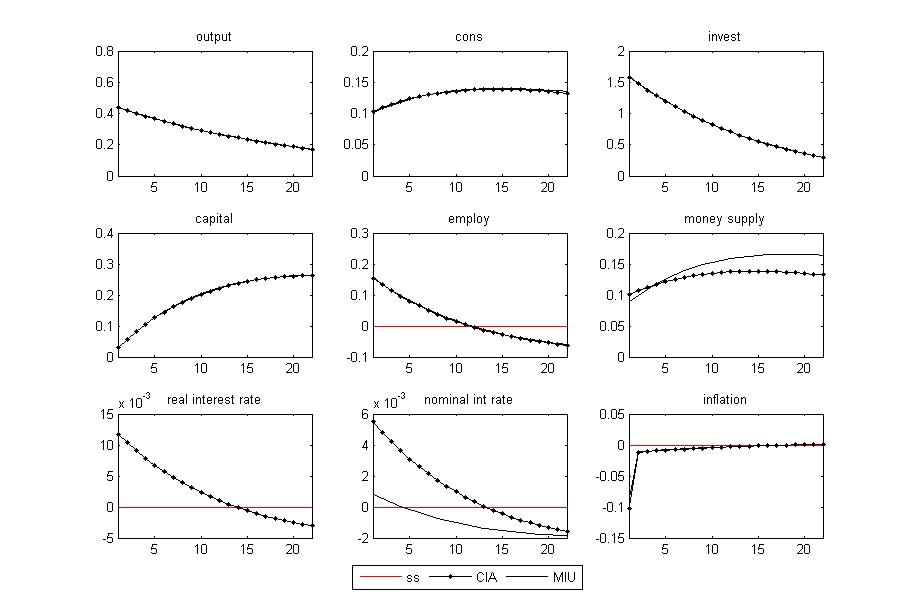
\includegraphics[width = 4.0in]{CIA-MIUtechshock.jpg}
\end{frame}

\begin{frame}
\frametitle{\small Dynamics (Impulse response to a money supply shock)}\footnote{{\tiny{To match CIA, share of money in utility 9 times larger. Contrary to calibration of 9 times smaller. This only has a visible impact on real variables; m , r , i, pi unaffected. Do you know why?}}}
\centering
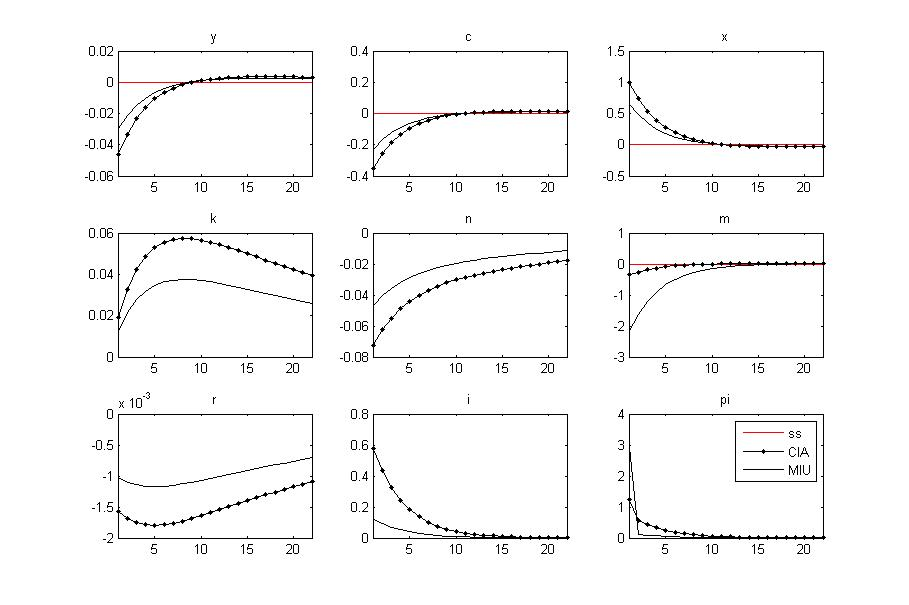
\includegraphics[width = 4.0in]{CIA-MIUmoneyshock.jpg}

\end{frame}


\section{Appendix}
\begin{frame}
\begin{center}
\Large{Appendix}
\end{center}
\end{frame}


\appendix

%\include{Assignment_money}

\renewcommand{\theequation}{A.\arabic{equation}}
\setcounter{equation}{0}

\section{Appendix A: Steady States}

\begin{frame}
\frametitle{Appendix A: Steady States} \vskip 0.1in

\textcolor{blue}{$\blacktriangleright$} $\frac{m^{ss}}{c^{ss}}$\\

From \eqref{Eq5.25} we have:

\begin{equation}\label{Eq5a.1}
\frac{m_{t}}{c_{t}} = (\frac{a}{1-a})^{-\frac{1}{\eta_{m}}}
(\frac{i_{t}}{1+i_{t}})^{-\frac{1}{\eta_{m}}}
\end{equation}

Since $1+i^{ss}=R^{ss}(1+\pi^{ss})$ and $R^{ss}=\frac{1}{\beta}$, in
steady state:

\begin{equation}\label{Eq5a.2}
(\frac{i^{ss}}{1+i^{ss}})= (\frac{1+\pi^{ss}-\beta}{1+\pi^{ss}})
\end{equation}

Substitute \eqref{Eq5a.2} into \eqref{Eq5a.1},

\begin{equation}\label{Eq5a.3}
\frac{m^{ss}}{c^{ss}} = (\frac{a}{1-a})^{-\frac{1}{\eta_{m}}}
(\frac{1+\pi^{ss}-\beta}{1+\pi^{ss}})^{-\frac{1}{\eta_{m}}}
\end{equation}

\end{frame}



\begin{frame}
\frametitle{Appendix A: Steady States} \vskip 0.1in

\textcolor{blue}{$\blacktriangleright$} $\tilde{C}^{ss}$\\

In steady state,

\begin{eqnarray}
\tilde{C}^{ss} &=& a (c^{ss})^{1-\eta_{m}}+
(1-a)(m^{ss})^{1-\eta_{m}}
\label{Eq5a.4}\\
\tilde{C}^{ss} &=& a (c^{ss})^{1-\eta_{m}}+ (c^{ss})^{1-\eta_{m}}
(1-a)(\frac{m^{ss}}{c^{ss}})^{1-\eta_{m}} \label{Eq5a.5}
\end{eqnarray}

Substitute \eqref{Eq5a.3} into \eqref{Eq5a.5},

{\scriptsize{
\begin{eqnarray}
\tilde{C}^{ss} &=& a (c^{ss})^{1-\eta_{m}}+ (c^{ss})^{1-\eta_{m}}
(1-a)[(\frac{a}{1-a})^{-\frac{1-\eta_{m}}{\eta_{m}}}
(\frac{1+\pi^{ss}-\beta}{1+\pi^{ss}})^{-\frac{1-\eta_{m}}{\eta_{m}}}] \label{Eq5a.6}\\
\tilde{C}^{ss} &=& a (c^{ss})^{1-\eta_{m}}[1+(\frac{1-a}{a})
(\frac{a}{1-a})^{\frac{\eta_{m}-1}{\eta_{m}}}
(\frac{1+\pi^{ss}-\beta}{1+\pi^{ss}})^{\frac{\eta_{m}-1}{\eta_{m}}}] \label{Eq5a.7}\\
\tilde{C}^{ss} &=& a (c^{ss})^{1-\eta_{m}}[1+
(\frac{a}{1-a})^{\frac{-1}{\eta_{m}}}
(\frac{1+\pi^{ss}-\beta}{1+\pi^{ss}})^{\frac{\eta_{m}-1}{\eta_{m}}}]
\label{Eq5a.8}
\end{eqnarray}}}

\end{frame}


\begin{frame}
\frametitle{Appendix A: Steady States} \vskip 0.1in

\textcolor{blue}{$\blacktriangleright$} $n^{ss}$\\

From the FOC with respect to $n_{t}$ \eqref{Eq5.15}, we know:
\begin{eqnarray}
U_{n}(c_{t},m_{t},1-n_{t}) &=&
U_{c}(c_{t},m_{t},1-n_{t})f_{n}(k_{t-1},n_{t},z_{t})
\label{Eq5a.9}\\
\frac{(1-n_{t})^{-\eta_{n}}}{a c_{t}^{-\eta_{m}}
\tilde{C}_{t}^{\frac{\eta_{m}-\eta_{c}}{1-\eta_{m}}}} &=&
(1-\alpha)\frac{y_{t}}{n_{t}}\label{Eq5a.10}
\end{eqnarray}

In steady state, we have:

\begin{equation}\label{Eq5a.11}
(1-n^{ss})^{-\eta_{n}}=a
(c^{ss})^{-\eta_{m}}(1-\alpha)(\frac{y^{ss}}{n^{ss}})(\tilde{C}^{ss})^{\frac{\eta_{m}-\eta_{c}}{1-\eta_{m}}}
\end{equation}

\end{frame}

\begin{frame}
\frametitle{Appendix A: Steady States} \vskip 0.1in

\textcolor{blue}{$\blacktriangleright$} $n^{ss}$\\

{\scriptsize{
Making use of the steady state values of
$\tilde{C}^{ss}$, $\frac{y^{ss}}{k^{ss}}$, and
$\frac{n{ss}}{k^{ss}}$,


\begin{eqnarray}
(1-n^{ss})^{-\eta_{n}} &=& a
(c^{ss})^{-\eta_{m}}(1-\alpha)(\frac{y^{ss}}{k^{ss}})^{\frac{-\alpha}{1-\alpha}}
\nonumber\\&& \{a (c^{ss})^{1-\eta_{m}}[1+
(\frac{a}{1-a})^{\frac{-1}{\eta_{m}}}
(\frac{1+\pi^{ss}-\beta}{1+\pi^{ss}})^{\frac{\eta_{m}-1}{\eta_{m}}}]
\}^{\frac{\eta_{m}-\eta_{c}}{1-\eta_{m}}} \label{Eq5a.12}\\
(1-n^{ss})^{-\eta_{c}} &=& a^{\frac{1-\eta_{c}}{1-\eta_{m}}}
(c^{ss})^{-\eta_{c}}(1-\alpha)(\frac{y^{ss}}{k^{ss}})^{\frac{-\alpha}{1-\alpha}}
\nonumber\\&& [1+ (\frac{a}{1-a})^{\frac{-1}{\eta_{m}}}
(\frac{1+\pi^{ss}-\beta}{1+\pi^{ss}})^{\frac{\eta_{m}-1}{\eta_{m}}}]
^{\frac{\eta_{m}-\eta_{c}}{1-\eta_{m}}}\label{Eq5a.13}
\end{eqnarray}

Replacing $(c^{ss})^{-\eta_{c}}$ with
$(\frac{c^{ss}}{k^{ss}})^{-\eta_{c}}
(\frac{k^{ss}}{n^{ss}})^{-\eta_{c}} (n^{ss})^{-\eta_{c}}$, we have:

\begin{eqnarray}\label{Eq5a.14}
\frac{(n^{ss})^{\eta_{c}}}{(1-n^{ss})^{\eta_{c}}} &=&
a^{\frac{1-\eta_{c}}{1-\eta_{m}}}
(1-\alpha)(\frac{y^{ss}}{k^{ss}})^{\frac{-\alpha}{1-\alpha}}
(\frac{c^{ss}}{k^{ss}})^{-\eta_{c}}
(\frac{k^{ss}}{n^{ss}})^{-\eta_{c}} \nonumber\\&& [1+
(\frac{a}{1-a})^{\frac{-1}{\eta_{m}}}
(\frac{1+\pi^{ss}-\beta}{1+\pi^{ss}})^{\frac{\eta_{m}-1}{\eta_{m}}}]
^{\frac{\eta_{m}-\eta_{c}}{1-\eta_{m}}}
\end{eqnarray}
}}

\end{frame}



\end{document}
